\documentclass[12pt,a4paper]{article}
\usepackage{tabularx}
\usepackage[utf8]{inputenc}
\usepackage[english]{babel}
\usepackage{amsmath}
\usepackage{amsfonts}
\usepackage{amssymb}
\usepackage{graphicx}
\usepackage{mathtools}
\usepackage{amsfonts}
\usepackage{subcaption}
\usepackage[linktocpage]{hyperref}
\usepackage[bottom]{footmisc}
\usepackage{float}
%\usepackage{cite}
\usepackage{commath}
%code insert
\usepackage{listings}
\usepackage[framed,numbered,autolinebreaks,useliterate]{mcode}
%pict insert
\usepackage{graphicx}
\usepackage[export]{adjustbox}
%
\usepackage[left=2cm,right=2cm,top=2cm,bottom=2cm]{geometry}
\everymath{\displaystyle}
\author{Eva María Urbano González, Pol Fontanes, Boyan Naydenov}
\title{Parametrització d'un motor Jet}


\begin{document}
\begin{titlepage}
	\centering
	\vspace{4.5cm}
	{\scshape ESEIAAT \par}
	{\scshape\Large Sistemes de Propulsió d'Aeronaus \par}
	\vspace{1.5cm}
	{\huge\bfseries Parametrització d'un motor Jet \par}
	\vspace{15cm}
	{\Large\itshape Eva María Urbano González\par}
	{\Large\itshape Pol Fontanes\par}
	{\Large\itshape Boyan Naydenov\par}
	\vfill
	\vspace{1cm}
	\today
\end{titlepage}
\tableofcontents
\lstlistoflistings
\listoffigures
\pagebreak
\section{Introducció i Objectius}
El present treball forma part de l'assignatura de Sistemes de Propulsió d'Aeronaus. Gran part d'aquesta assignatura consisteix en l'estudi dels tipus de motors d'una aeronau i de les possibilitats d'optimització, a més de la parametrització dels motors tant en cas ideal com en cas real.\\
Per tal profunditzar en les àrees de coneixement relacionades amb l'assignatura es proposa la realització d'aquest projecte. L'objectiu es el disseny preliminar de la motorització d'una aeronau partint de tres condicions de disseny: empenta, velocitat i altitud de vol. Amb aquestes condicions el sistema no queda definit, de manera que es necessari establir certs criteris per a aconseguir tots els paràmetres del motor. En les següents pàgines es discutirà quin tipus de motor pot ser adequat i el criteri de disseny a utilitzar.\\
A més de fer el càlcul del motor escollit, es faran estudis per a la possible implementació de \textit{mixer}, \textit{propeller} i \textit{afterburner}. Amb aquests estudis es busca saber si pel motor escollit aquests sistemes son profitosos o no, tenint en compte els resultats obtinguts amb ells i sense ells i el pensament crític del grup de treball.\\
Per últim es discutirà com serà el motor final i es calcularan les àrees d'aquest i el consum d'aire i combustible.\\
Els càlculs que es mostraran han estat realitzats utilitzant un codi desenvolupat en MATLAB. Aquest codi ha sigut verificat utilitzant com a referencia problemes resolts a classe\footnote{Verificació del codi es pot visualitzar a l'Annex B} per a assegurar la validesa dels resultats. El codi es pot visualitzar a l'Annex A. La informació teòrica per a poder-lo fer a estat extreta dels apunts de classe de teoria i problemes de l'assignatura de Sistemes de Propulsió d'Aeronaus tant per part de Pau Manent com per part de Marc Maymó i del llibre \textit{Elements of Gas Turbine Propulsion}, de Jack D. Mattingly. 
\section{Descripició del/s motor/s}
\label{descripcio}
Les característiques que ha de complir el motor son les següents:
\begin{itemize}
\item Empenta de creuer: $F=25000N$
\item Alçada de vol: $h=9500m$
\item Velocitat de creuer: $v=600km/h$
\end{itemize}
A més de tot això es tracta d'un disseny real, per la qual cosa s'han de tenir en compte els següents ratis i temperatura màxima d'entrada a la turbina:
\begin{itemize}
\item Rati de pressió al difusor: $\pi_d=0.96$
\item Rendiment al compressor: $\eta_c=0.88$
\item Rati de pressió a la cambra de combustió: $\pi_b=0.94$
\item Eficiència de combustió: $\eta_b=0.99$
\item Rendiments de turbina: $\eta_{tH}=\eta_{tL}=0.87$
\item Rati de pressió a la tovera: $\pi_n=0.98$
\item Rendiment mecànic: $\eta_{mec}=0.99$
\item Temperatura d'entrada a la turbina: $T_{t4}=1780$
\end{itemize}
Segons la Figura \ref{operacio}, per a les característiques esmentades els millors candidats serien el turbojet i el turbofan.
\begin{figure}[h]
\centering
\includegraphics[width=0.5\textwidth]{./pics/seleccio.JPG} 
\caption{Operació motors d'aeronaus. Imatge extreta de \cite{mattingly}.}
\label{operacio}
\end{figure}
Un dels criteris per al disseny del motor serà el de minimitzar el consum de combustible incrementant l'eficiència propulsiva. El tipus de motor adequat es doncs el turbofan,  més massa a una velocitat més petita. 
\section{Elecció de les condicions de disseny}
Donada l'alçada i la velocitat de vol, així com $T_{t4}$ les tres variables necessàries per fer el disseny són $\pi_c$, $\pi_f$ i $\alpha$. Aquests s'han d'escollir per tal d'obtenir el millor motor possible donades les dades de l'enunciat mostrades a l'apartat \ref{descripcio}.
La definició dels paràmetres de disseny es:
\begin{equation*}
	\pi_c = \frac{P_{3t}}{P_{2t}} = \pi_{f}\times\pi_{cL} = \frac{P_{2.5t}}{P_{2t}} \times \frac{P_{3t}}{P_{2.5t}}
\end{equation*}
\begin{equation*}
	\pi_f = \frac{P_{2.5t}}{P_{2t}} = \frac{P_{1.3t}}{P_{2t}} 
\end{equation*}
\begin{equation*}
	\alpha = \frac{m_{primari}}{m_{secundari}}
\end{equation*}
\noindent Per fer la tria,  s'ha fet un extens estudi amb l'objectiu de trobar els paràmetres adequats a les condicions de vol proporcionades a l'enunciat i als criteris de disseny imposats. Aquests es troben integrat a la funció \textit{opt\_parametros.m}, que prova diferents combinacions de $\pi_f$ i $\pi_c$ i calcula amb elles la força adimensional. Es busca maximitzar aquest paràmetre per poder obtenir un motor petit. Tal i com es veu a la Figura \ref{Fadimensional}, al incrementar $\pi_f$ i $\pi_c$ també incrementa \(\hat{F}\) i no es possible calcular cap màxim. S'adopta la idea de que, quan al augmentar els valors de $\pi_f$ i $\pi_c$, \(\hat{F}\) no incrementa més d'un 5\% no val la pena continuar augmentant els ratis de compressió.
\begin{figure}[H]
	\centering
	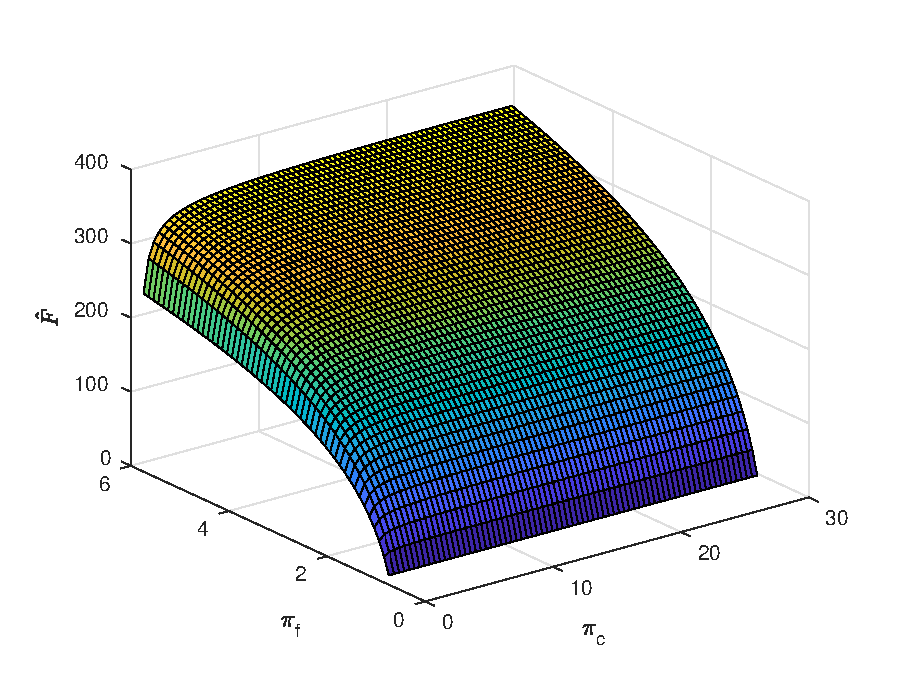
\includegraphics[width=0.35\textwidth]{./pics/F_pc_pf}
	\caption{\(\hat{F}\) en funció de $\pi_c$ i $\pi_f$}
	\label{Fadimensional}
\end{figure}
A més de maximitzar la força adimensional, es vol garantir un consum específic mínim. Per cada combinació  $\pi_f$ i $\pi_c$ de valors, es pot obtenir la $\alpha$ corresponent per complir aquest requisit, seguint el procediment proposat a \cite[5-10]{mattingly} que principalment es basa en imposar:
\begin{equation*}
	\frac{\partial S}{\partial \alpha} = 0 
\end{equation*}
Arribant així a:
\begin{multline}
	\alpha_{opt} = \frac{1}{\tau_r(\tau_f-1)}\bigg[\tau_{\lambda}-\tau_r(\tau_c-1)-\frac{\tau_{\lambda}}{\tau_r\tau_c} \\ -\frac{1}{4}(\sqrt{\tau_r\tau_f-1} + \sqrt{\tau_r-1})^2\bigg]
\end{multline}
\begin{figure}[H]
	\centering
	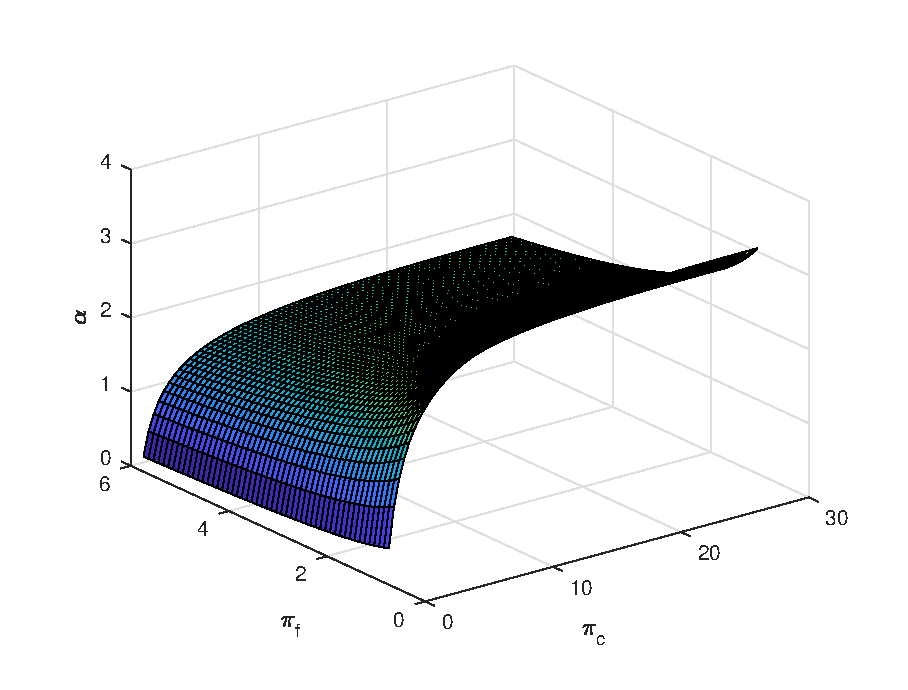
\includegraphics[width=0.35\textwidth]{./pics/alpha_pc_pf}
	\caption{$\alpha_{opt}$ en funció de $\pi_c$ i $\pi_f$}
\end{figure}
Finalment, els valors obtinguts són els següents:
\begin{figure}[H]
	\centering
	\begin{tabular}{lc}
		\toprule[3pt]
		\textbf{Paràmetre}&\textbf{Valor}\\
		\midrule[1pt]
		$\pi_{c}$ & 22.60 \\
		$\pi_{f}$ & 2.20 \\
		$\alpha_{opt}$ & 2.35 \\
		\bottomrule[2pt]
	\end{tabular}
	\label{C_opti2}
	\caption{Selecció dels paràmetres de disseny}
\end{figure}
\noindent Aquests s'han comparat a valors típics d'altres aeronaus i s'ha conclòs que són uns valors raonables i realistes. Tot el procés realitzat es pot veure esquematitzat a la Figura \ref{opt}.
Resumidament, s'ha anat variant $\pi_c$ o $\pi_f$ fins arribar a una convergència de valors que donés un increment no significatiu de $\hat{F}$. 
\begin{figure}[H]
	\centering
	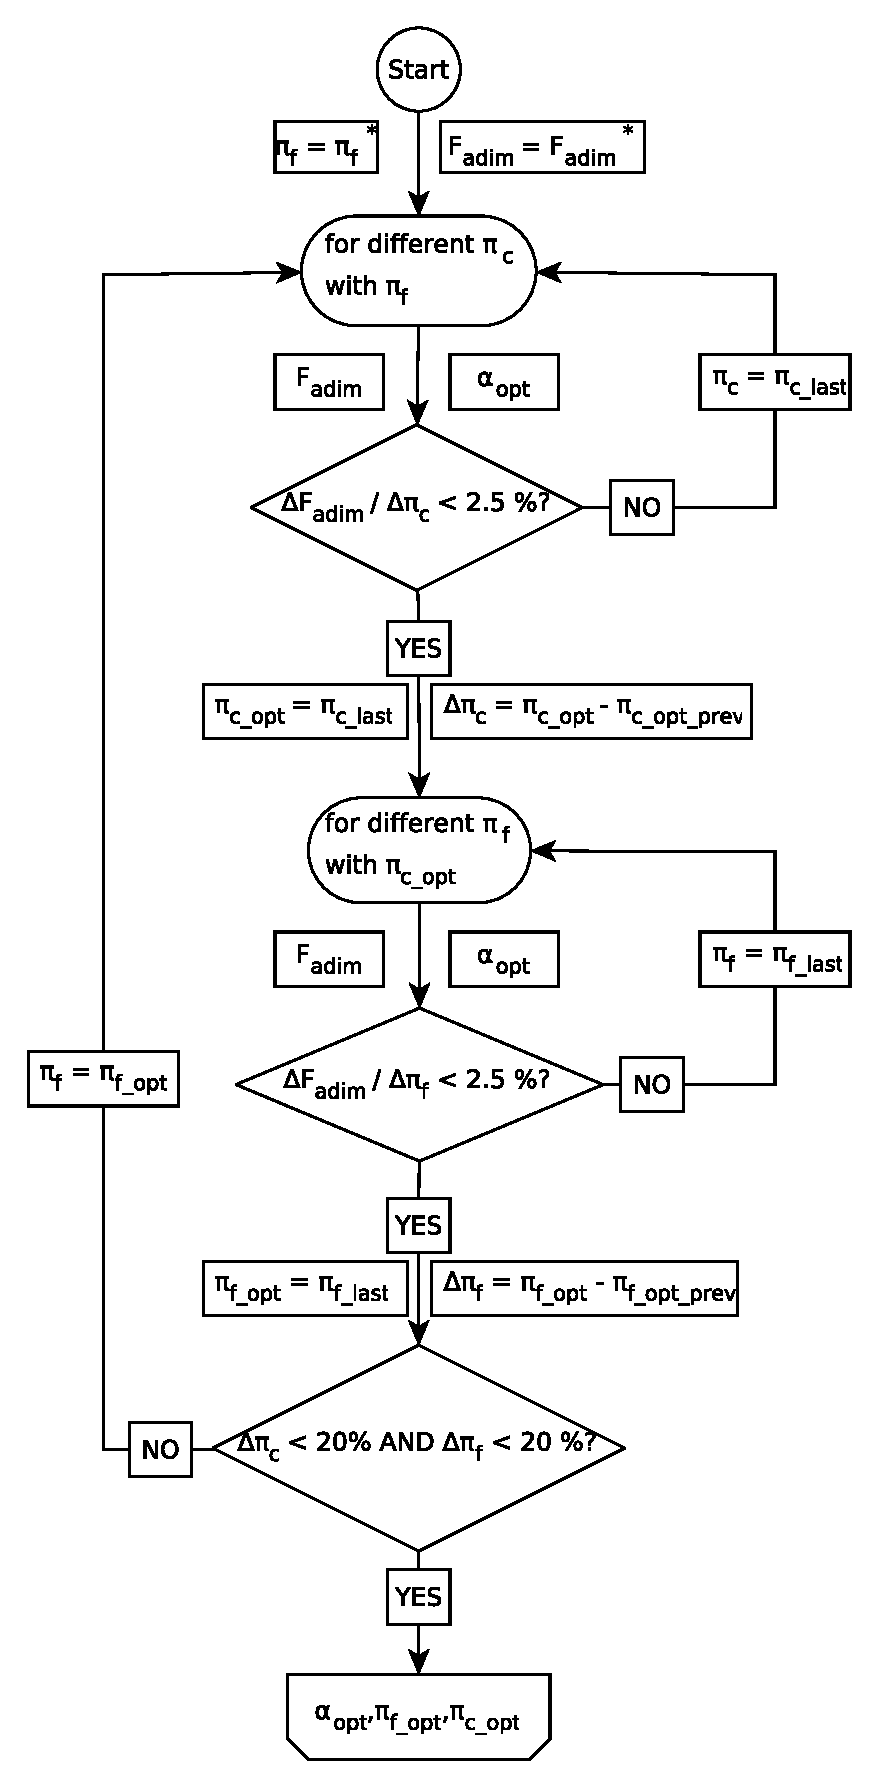
\includegraphics[scale=0.6]{./pics/optimization}
	\caption{Algoritme emprat per trobar els valors òptims}
	\label{opt}
\end{figure}
\section{Càlcul paramètric del motor real}
El següent pas consisteix a resoldre el turbofan real sencer, sense tindre en compte \textit{mixer} ni \textit{afterburner}, obtenint així la distribució de pressions, temperatures i fluxos màssics. A continuació es mostren algunes consideracions rellevants per a cada etapa \footnote{La I indica ideal mentre que la R, real.}:
\begin{itemize}
\item \textbf{0t - 2t: Difusor}. Es considera adiabàtic i per tant, $\tau_d = 1$. Per altra banda si que es produeix una pèrdua de pressió total que es manifesta com $\pi_d = \eta_d$.
\item \textbf{2t - 2.5t: Fan}. Com que la tasca primordial del fan es incrementar la pressió, es fixa la pressió que assoleix el compressor ideal i es dissenya el cas real per tal que assoleixi el mateix objectiu, es a dir, la pressió de sortida es manté constant però la temperatura varia segons la eficiència. Així, $P_{t25}^R = P_{t25}^I$ tot i que $T_{t25}^R \neq T_{t25}^I$ . Coneixent el rendiment $\eta_f$ es troben les noves temperatures.
\item \textbf{2.5t - 3t: Compressor de baixa}. La mateixa explicació del fan és vàlida per al compressor de baixa doncs es dissenya amb el mateix criteri.
\item \textbf{3t - 4t: Cambra de combustió}. En un cas ideal la combustió es produeix de forma isòbara mentre que al cas real hi ha una pèrdua de pressió total. Ds dissenya per tal d'arribar a la $T_{t4}$ de disseny. El consum de combustible es troba igualant la calor generada per la crema a la calor proporcionada al fluid. Es important esmentar que en la realització del codi no s'han fet simplificacions com considerar $C_P=ct$ o $(1+f)\simeq1$.
\item \textbf{4t - 4.5t: Turbina d'alta}. L'objectiu de la tovera real serà el d'aconseguir expandir el fluid per tal d'aportar el treball necessari al compressor. Per resoldre la turbina doncs, cal igualar treballs. Concretament: $\dot{W_{cH}^R} = \dot{W_{tH}^R} $. D'aquesta igualtat s'obté $\tau_{tH}^R$ que si es combina amb $\eta_{tH}$ s'obté $\tau_{tH}^I$ que permet trobar  $P_{tH}^{I} = P_{tH}^{R}$.
\item \textbf{4.5t - 6t: Turbina de baixa}. La mateixa explicació de la turbina d'alta serveix per la de baixa, amb la diferència que ara el treball s'iguala al del fan.
\item \textbf{6t - 9t: Tovera Primari}. Es considera adiabàtica i per tant, $\tau_n = 1$. Per altra banda, $\pi_n = \eta_n$. Per últim, per trobar els valors dinàmics a la sortida, es suposa que la tovera està adaptada ($P_9 = P_0$) i si no ho està es restringeix el valor $M_9=1$ ja que considerem tovera convergent.
\item \textbf{16t - 19t: Tovera Secundari}. Funciona exactament igual que la del primari però amb les condicions d'entrada del flux secundari.
\end{itemize}
Finalment, els resultats obtinguts que dóna el programa \textbf{MAIN\_TURBOFAN.m} amb les opcions de \textit{mixer}, \textit{afterburner} i \textit{propeller} desactivades són:
\begin{table}[H]
\centering
\begin{tabular}{lcccc}
\toprule[3pt]
\textbf{Etapa} &\textbf{$\bm{\pi}$} & \textbf{$\bm{\tau}$}    & \textbf{Pt} [kPa]  & \textbf{Tt} [K]  \\
\midrule[1pt]
0 - 0t     & 1.23   & 1.06  & 35.10   & 240.22             \\
0t - 2t     & 0.96   & 1  & 33.70   & 240.22             \\
2t - 2.5t/13t     & 2.20   & 1.29  & 74.13   & 309.20             \\
2.5t - 3t     & 10.27  & 2.07  & 761.52   & 641.44             \\
3t - 4t     & 0.94     & 0.76  & 715.83  & 1780.00             \\
4t - 4.5t     & 0.43   & 0.85  & 311.23   & 1509.20             \\
4.5t - 6t     & 0.51   & 0.88  & 159.00   & 1320.70             \\
6t - 9t     & 0.98   & 0.92  & 155.81   & 1320.70            \\
16t - 19t     & 0.98   & 0.92  & 72.65   & 309.20            \\
\bottomrule[2pt]
\end{tabular}
\caption{Pressions i Temperatures - motor real}
\end{table}
Pel que fa als fluxos màssics:
\begin{figure}[H]
	\centering
	\begin{tabular}{lc}
		\toprule[3pt]
		\textbf{Paràmetre}&\textbf{Valor [kg/s]}\\
		\midrule[1pt]
		$m_{o}$ & 15.06 \\
		$m_{sec}$ & 35.46 \\
		$m_{f}$ & 0.56 \\
		\bottomrule[2pt]
	\end{tabular}
	\label{C_opti2}
	\caption{Fluxos màssics - motor real}
\end{figure}
Per aquesta configuració s'obté una empenta adimensonal de $\bm{\hat{F} = 5.5}$.
\section{Càlcul i elecció de l'hèlix}
Per el·legir una hèlix, cal calcular el turboprop que la mourà. Aleshores, el turbofan dissenyat anteriorment, a nivell pràctic, se l'hi extraurà el fan per substituir-lo per una hèlix. 
\clearpage
\section{Càlcul i elecció de postcombustor}
Com s'ha vist amb anterioritat, el mixer pe'ls nostres paràmetres donava problemes a l'implementar-lo. Així doncs, es decideix calcular un postcombustor que només vagi adherit al core del turbofan, creant la postcombustió del flux primari.

\subsection{Paràmetres suposats }
Tot i que la gran majoria de paràmetres venien donats per l'enunciat del treball, amb l'objectiu de fer-lo més realista s'han suposat certes eficiències específiques del component estudiat.

\begin{figure}[H]
	\centering
	\begin{tabular}{lc}
		\toprule[3pt]
		\textbf{Paràmetre}&\textbf{Valor}\\
		\midrule[1pt]
		$\gamma_{AB}$ & $1.3$\\
		$ Cp_{AB}$ & $Cp_c$\\
		$T_{t7}$ & $2400K$\\
		$\eta_{AB}$ & $0.99$\\
		
		\bottomrule[2pt]
	\end{tabular}
	\label{ABparam}
	\caption{Paràmetres suposats al postcombustor.}
\end{figure}


\subsection{Postcombustor adherit al flux primari}
Per calcular el postcombustor, s'ha seguit la referencia dels problemes solucionats per Pau Manent a l'assignatura i la referencia del llibre \cite{mattingly}.\\

\noindent Es comença, solucionant el cas del turbofan real com en els apartats anteriors, fins obtenir els valors dels seus paràmetres a les toveres.

\noindent Després, comença el càlcul del postcombustor, situat al final de la turbina. Es considera que $T_{t9} = T_{t7}$, $P_{t9}=\pi_nP_{t6}$ i es defineix $\tau_{\lambda AB} = \frac{Cp_{AB}T_{t7}}{Cp_cT_0}$.

\noindent Aleshores, es calcula la fracció de massa de combustible ($f_{AB}=\dot{m}_{fAB}/\dot{m}_0$) que el postcombustor afegeix al flux primari.

\begin{equation}
	f_{AB}=(1+f)\frac{\tau_{\lambda AB}-\tau_{\lambda}\tau_t}{\eta_{AB}\frac{h}{Cp_cT_0}-\tau_{\lambda AB}}
\end{equation}
 
 
\noindent Finalment, les seccions situades després del postcombustor són recalculades, ja que, els paràmetres de sortida del postcombustor les modifica. Concretament s'imposa que $f = f +f_{AB}$ dins el codi per poder aplicar la funció de càlcul de la força adimensional (\textit{Fadimensional.m}). S'acaba el càlcul de l'afterburner extraient els cabals màssics característics del motor amb afterburner (\textit{Fluxosmasics.m}).

\subsubsection{Resultats postcombustor}
\begin{figure}[H]
	\centering
	\begin{tabular}{lcc}
		\toprule[3pt]
		\textbf{Paràmetre}&\textbf{Valor amb AB}&\textbf{Valor sense AB}\\
		\midrule[1pt]
		$\hat{F}$ & $1.3$ & $1.3$\\
		$ \dot{m}_0$ & $Cp_c$ & $1.3$\\
		$T_{t7}$ & $2400K$ & $1.3$\\
		$\eta_{AB}$ & $0.99$ & $1.3$\\
		
		\bottomrule[2pt]
	\end{tabular}
	\label{ABres}
	\caption{Resultats d'implementar el postcombustor.}
\end{figure}


\clearpage


\section{Càlcul de consum d’aire i fuel en vol}

\section{Càlcul de dimensionat d’àrees}


\newpage
\bibliographystyle{unsrt}
\bibliography{Ingenieria_computacional}
\end{document}
